% !TEX root = ../main.tex
\section{Analysis of Basic Statistics} \label{sec:basicstatistics}

	\subsection{Background Information} \label{sec:summaryogbasicstats}

		%Table: Summary of the background information
		\begin{table}[H]
      \parbox{.45\linewidth}{
        \centering
        \begin{tabular}{ l | l l }
          \hline
          \multicolumn{3}{l}{\bf Respondents} \\ \hline
          Completed survey & 802 \\
          Stoped during survey & 11 \\
          Started creating patterns & 204 \\
          Opened survey and left & 81 \\ \hline
            
          \multicolumn{3}{l}{\bf Gender} \\ \hline
          Male & 529 & 66\% \\
          Female & 278 & 34\% \\ \hline

          \multicolumn{3}{l}{\bf Handedness} \\ \hline
          Left & 97 & 12\% \\
          Right & 690 & 88\% \\ \hline

          \multicolumn{3}{l}{\bf Experience with IT/Security} \\ \hline
          Yes & 470 & 59\% \\
          No & 332 & 41\% \\ \hline

          \multicolumn{2}{l}{\bf Reading/Writing direction} \\ \hline
          Top-to-bottom & 7 & 1\% \\
          Right-to-Left & 8 & 1\% \\
          Left-to-right & 792 & 98\% \\ \hline
        \end{tabular}
        \caption{Summary of the respondents}
        \label{tab:respondentsBasics}
      }
      \hfill
      \parbox{.45\linewidth}{
        \centering
        \vspace{1.7cm}
        \begin{tabular}{ l | l l }
          \hline
          \multicolumn{3}{l}{\bf Used Android Unlock Pattern} \\ \hline
          Yes & 526 & 65\% \\ 
          No & 278 & 35\% \\ \hline

          \multicolumn{3}{l}{\bf Use screenlock} \\ \hline
          Yes & 655 & 82\% \\
          No & 149 & 18\% \\ \hline

          \multicolumn{3}{l}{\bf Screenlock in use} \\ \hline
          Android Pattern Lock & 202 & 31\% \\
          4-digit PIN & 237 & 36\% \\
          Fingerprint & 116 & 18\% \\
          Password & 44 & 7\% \\
          slide-to-unlock & 28 & 4\% \\
          Other & 28 & 4\% \\ \hline
        \end{tabular}
        \caption{Screen lock habits}
        \label{tab:screenlockHabits}
      }
    \end{table}

    %Figure: Age distribution
    \begin{figure}[H]
      \centering
      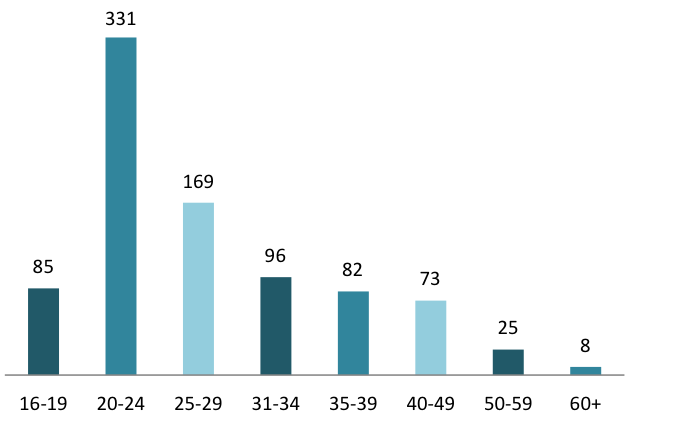
\includegraphics[scale=0.8]{pics/analysis/AgeDist.png}
      \caption{Age distribution}
      \label{fig:ageDistribution}
    \end{figure}

  \clearpage
	\subsection{Country of Origin} \label{sec:countryoforigin}

		%Table: Country of origin (39 countires)
		\begin{table}[H]
	    \centering
	    \begin{tabular}{ l c | c }
	      \hline
	      \multicolumn{2}{l}{Country} & \# Respondents \\ \hline
	      \raisebox{-.4\height}{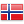
\includegraphics{pics/flags/Norway.png}} & Norway & 517 \\ \hline
	      \raisebox{-.4\height}{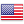
\includegraphics{pics/flags/USA.png}} & United States of America & 115 \\ \hline
	      \raisebox{-.4\height}{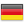
\includegraphics{pics/flags/Germany.png}} & Germany & 33 \\ \hline
	      \raisebox{-.4\height}{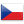
\includegraphics{pics/flags/CzechRepublic.png}} & Czech Republic & 31 \\ \hline
	      \raisebox{-.4\height}{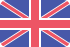
\includegraphics{pics/flags/UnitedKingdom.png}} & United Kingdom & 22 \\ \hline
	      \raisebox{-.4\height}{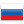
\includegraphics{pics/flags/Russia.png}} & Russia & 13 \\ \hline
	      \raisebox{-.4\height}{
\includegraphics{pics/flags/Denmark.png}} & Denmark & 7 \\ \hline
	      \raisebox{-.4\height}{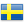
\includegraphics{pics/flags/Sweden.png}} & Sweden & 6 \\ \hline
	      \raisebox{-.4\height}{
\includegraphics{pics/flags/Switzerland.png}} & Switzerland & 6 \\ \hline
	      \raisebox{-.4\height}{
\includegraphics{pics/flags/Australia.png}} & Australia & 5 \\ \hline
	      \raisebox{-.4\height}{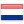
\includegraphics{pics/flags/Netherlands.png}} & Netherlands & 4 \\ \hline
	      \raisebox{-.4\height}{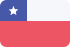
\includegraphics{pics/flags/Chile.png}} & Chile & 4 \\ \hline
	      \raisebox{-.4\height}{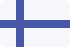
\includegraphics{pics/flags/Finland.png}} & Finland & 3 \\ \hline
	      \raisebox{-.4\height}{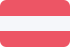
\includegraphics{pics/flags/Austria.png}} & Austria & 3 \\ \hline
	      \raisebox{-.4\height}{
\includegraphics{pics/flags/Ukraine.png}} & Ukraine & 3 \\ \hline
	      \raisebox{-.4\height}{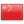
\includegraphics{pics/flags/China.png}} & China & 3 \\ \hline
	      \multicolumn{2}{p{7cm}|}{Afghanistan, Mexico, North Korea, Pakistan, Vietnam, Luxembourg, Ireland, Tunisia} & 2 \\ \hline
	      \multicolumn{2}{p{7cm} |}{Italy, Greece, Belgium, Indonesia, Malaysia, Bahrain, Botswana, Argentina, Singapore, japan, Canada, South Korea, Hungary, Turkey, Brazil} & 1 \\ \hline
	    \end{tabular}
	    \caption{Respondents country of origin}
	    \label{tab:country}
	  \end{table}
  
  \clearpage
	\subsection{Classification of Handsize} \label{sec:classificationhandsize}

		%Figure: Handsize
		\begin{figure}[H]
      \centering
      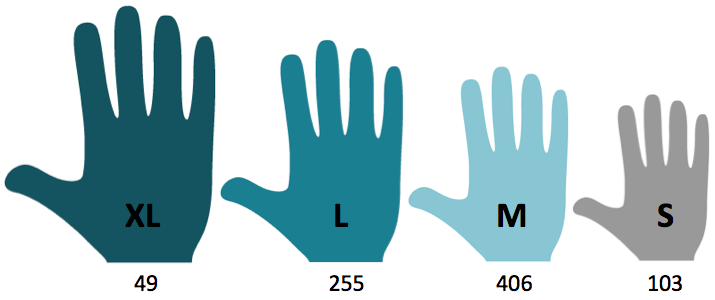
\includegraphics[width=0.8\textwidth]{pics/analysis/handsize.png}
      \caption{Handsize of all participants}
      \label{fig:handsize}
    \end{figure}

    %Table: Handsize and gender
    \begin{table}[H]
      \centering
      \begin{tabular}{ c || c | c | c | c || c }
        \hline
        & {\bf Xtra Large} & {\bf Large} & {\bf Medium} & {\bf Small} & {\bf Total}\\ \hline
        {\bf Male} & 45 (9\%) & 200 (38\%) & 246 (47\%) & 38 (7\%) & 529 \\
        {\bf Female} & 3 (1\%) & 54 (19\%) & 157 (56\%) & 64 (23\%) & 278 \\ \hline
      \end{tabular}
      \caption{Handsize and gender}
      \label{tab:HandsizeGender}
    \end{table}

  \clearpage
	\subsection{Classification of Screensize} \label{sec:classificationscreensize}

		%Figure: Iphone screensize distribution
		\begin{figure}[H]
      \centering
      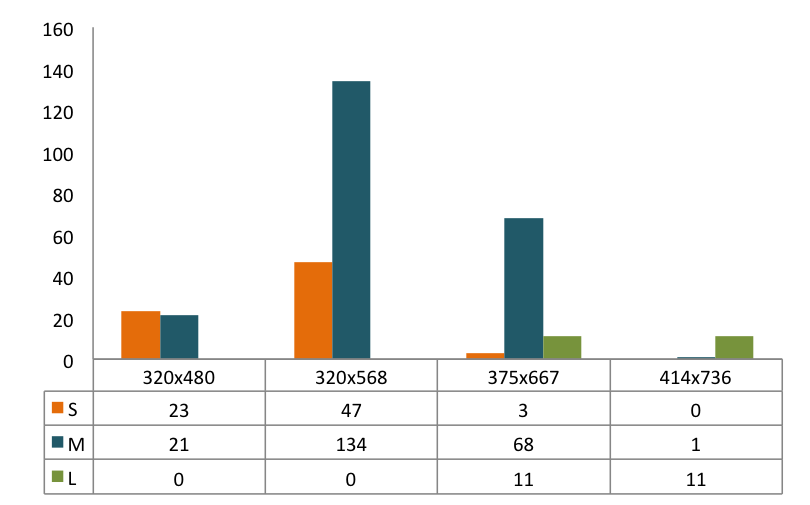
\includegraphics[scale=0.4]{pics/analysis/IphoneScreenDist.png}
      \caption{Iphone screensize distribution}
      \label{fig:iphoneScreenDist}
    \end{figure}
    
    %Table: Iphone Screen classification
    \begin{table}[H]
      \centering
      \begin{tabular}{ l | l | l }
        \hline
        {\bf Iphone Model}  & {\bf Resolution (px)} & {\bf Inches} \\ \hline
        iPhone 2G, 3G, 3GS, 4, 4s  &  320 $\times$ 480  &  3.5'' \\
        iPhone 5, 5s        &  320 $\times$ 568  &  4''   \\
        iPhone 6            &  320 $\times$ 568, 375 $\times$ 667  &  4.7'' \\
        iPhone 6 Plus       &  375 $\times$ 667, 414 $\times$ 736  &  5.5'' \\ \hline        
      \end{tabular}
      \caption{Iphone Screen classification}
      \label{tab:iphonescreen}
    \end{table}

  \clearpage
	\subsection{Created Patterns} \label{sec:createdpatterns}

		%Table: Starting node dist
		\begin{table}[H]
      \centering
      \begin{tabular}{ c || c | c || c | c | c | c }
        \hline
        {\bf Start node} & All & 1,2,3 & 1 & 2 & 3 & T \\ \hline
        1 & 44\% & 42\% & 43\% & 41\% & 42\% & 51\% \\
        3 & 15\% & 15\% & 16\% & 14\% & 13\% & 14\% \\
        7 & 14\% & 14\% & 13\% & 15\% & 14\% & 13\% \\
        2 & 9\%  & 9\%  & 10\% & 9\%  & 8\%  & 7\%  \\
        4 & 6\%  & 7\%  & 6\%  & 7\%  & 7\%  & 6\%  \\
        5 & 4\%  & 4\%  & 4\%  & 4\%  & 4\%  & 3\%  \\
        9 & 4\%  & 4\%  & 3\%  & 3\%  & 5\%  & 3\%  \\
        8 & 2\%  & 3\%  & 2\%  & 3\%  & 3\%  & 2\%  \\
        6 & 2\%  & 2\%  & 2\%  & 2\%  & 3\%  & 2\%  \\ \hline
      \end{tabular}
      \caption{Starting node (1 = Shopping, 2 = Smartphone, 3 = Bank, T = Training)}
      \label{tab:startingNode}
    \end{table}

    %Figure: Staring node for all patterns
    \begin{figure}[H]
      \centering
      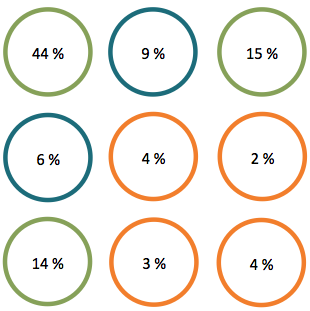
\includegraphics[scale=0.45]{pics/analysis/startingNode.png}
      \caption{Staring node for all patterns}
      \label{fig:startingNode}
    \end{figure}

    %Figure: Number of unique patterns
    \begin{figure}
      \centering
      \begin{minipage}[b]{0.40\linewidth}
      \centering
        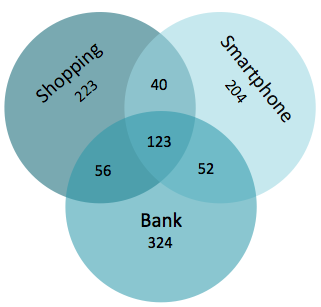
\includegraphics[scale=0.4]{pics/analysis/uniquePatternsVenn.png}
      \end{minipage}%
      \begin{minipage}[b]{0.30\linewidth}
        \centering
        \begin{tabular}{ c | c }
          \hline
          Shopping &  442 \\
          Smartphone & 419 \\
          Bank & 555 \\
          Training & 414 \\ \hline \hline
          All types & 1196 \\ \hline
        \end{tabular}
        \vspace{1cm}
      \end{minipage}
      \caption{Number of unique patterns}
      \label{fig:test}
    \end{figure}

    %Table: typing habits
    \begin{table}[H]
      \parbox{.5\linewidth}{
        \centering
        \begin{tabular}{ l | l | l }
          \hline
          {\bf Mobile held in} & {\bf Finger used} & {\bf \#} \\ \hline
          \multirow{3}{*}{Right} & Thumb & 366 \\
          & Forefinger & 41 \\
          & Other & 8 \\ \hline
          \multirow{3}{*}{Left} & Thumb & 33 \\
          & Forefinger & 217 \\
          & Other & 23 \\ \hline
        \end{tabular}
        \caption{{\bf Right-handed} typing habits}
        \label{tab:righthandfinger}
      }
      \hfill
      \parbox{.5\linewidth}{
        \centering
        \begin{tabular}{ l | l | l }
          \hline
          {\bf Mobile held in} & {\bf Finger used} & {\bf \#} \\ \hline
          \multirow{3}{*}{Right} & Thumb & 26 \\ 
          & Forefinger & 10 \\
          & Other & 4 \\ \hline
          \multirow{3}{*}{Left} & Thumb & 22 \\ 
          & Forefinger & 26 \\
          & Other & 6 \\ \hline
        \end{tabular}
        \caption{{\bf Left-handed} typing habits}
        \label{tab:lefthandfinger}
      }
    \end{table}

    %Figure: Average pattern creation time (seconds) and Pattern Length (nodes)
    \begin{figure}[H]
      \centering
      \subfigure[Average pattern creation time (seconds)]{
        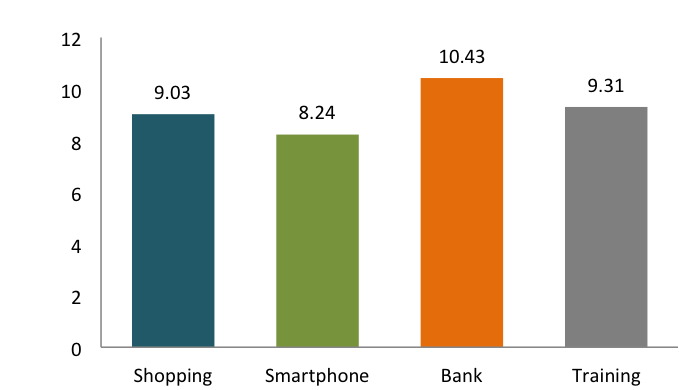
\includegraphics[scale=0.63]{pics/analysis/avgCreationTime.png}
      }
      \subfigure[Average Pattern Length (nodes)]{
        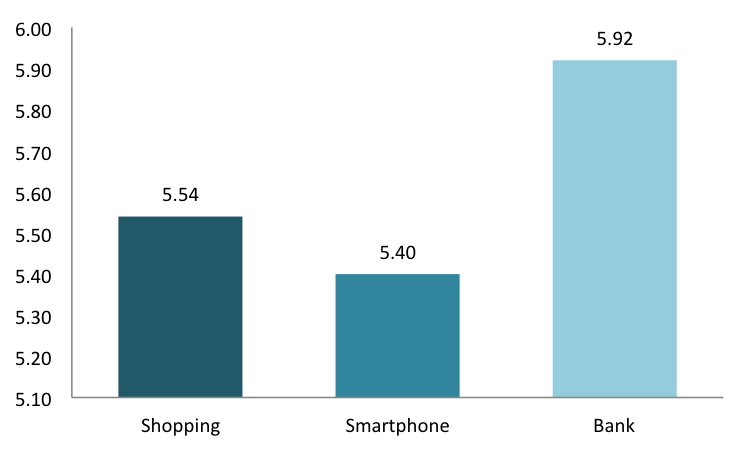
\includegraphics[scale=0.53]{pics/analysis/avgPatternLength.png}
      }
      \label{fig:creationTime}
    \end{figure}

    %Figure: Pattern Length distribution
    \begin{figure}[H]
      \centering
      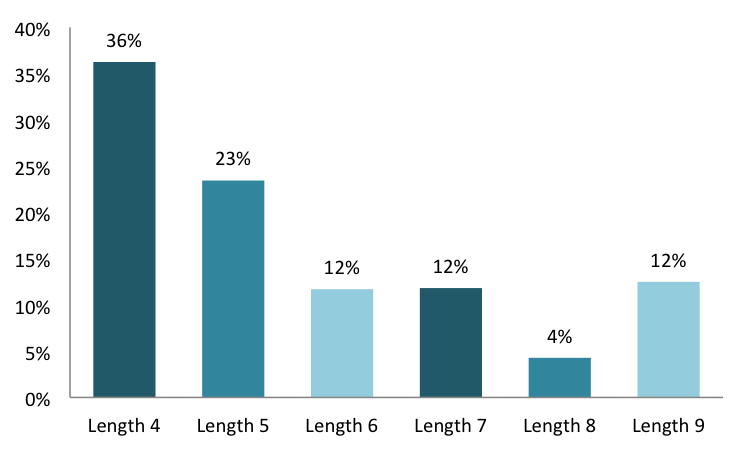
\includegraphics[scale=0.5]{pics/analysis/patternLength.png}
      \caption{Pattern Length distribution}
      \label{fig:patternLength}
    \end{figure}

    %Figure:Pattern length and type distribution
    \begin{figure}[H]
      \centering
      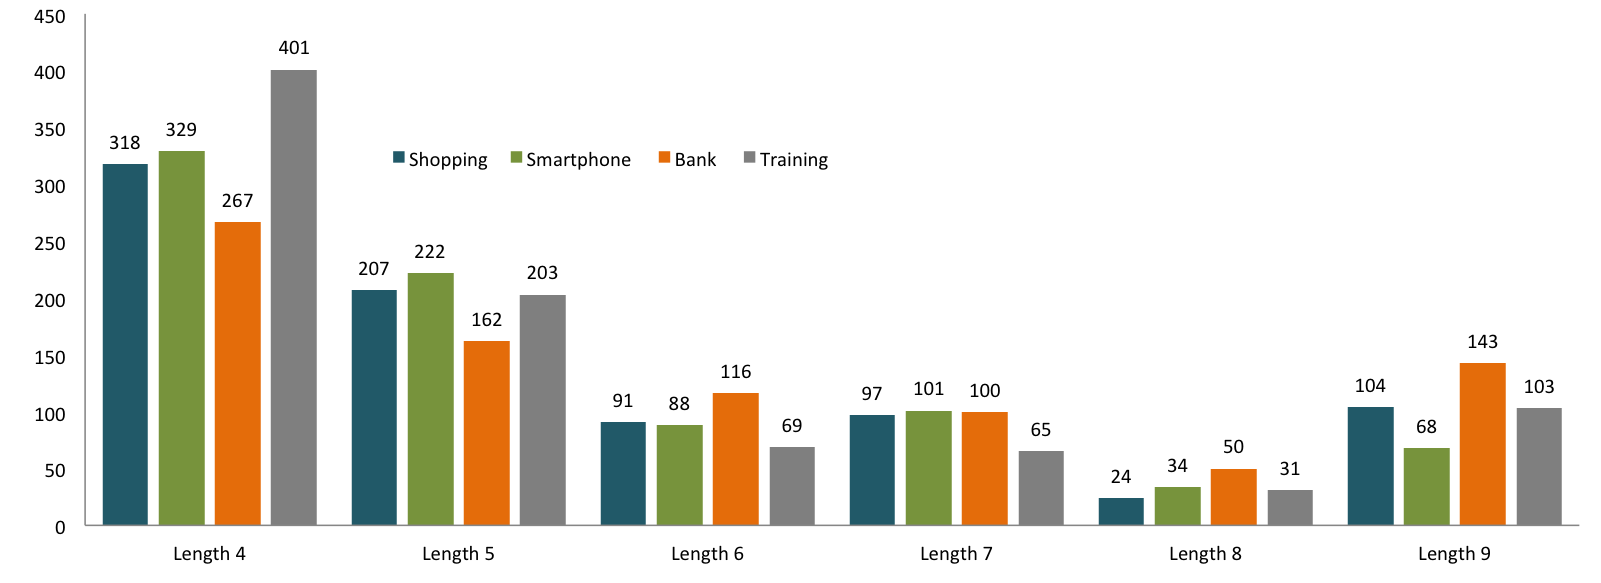
\includegraphics[width=\textwidth]{pics/analysis/patterntypePatternLength.png}
      \caption{Pattern length and type distribution}
      \label{fig:patternTypePatternLength}
    \end{figure}

    %Table: Top 20 patterns and number of appearances
    \begin{table}[H]
	    \centering
	    \begin{tabular}{l || l l | l l | l l | l l }
	      \hline
	      {\bf \#} & \multicolumn{2}{c|}{\bf Shopping} & \multicolumn{2}{c|}{\bf Smartphone} & \multicolumn{2}{c|}{\bf Bank} & \multicolumn{2}{c}{\bf Training} \\ \hline
	      1  & 1478      & 26 & 14789      & 27 & 14789      & 17 & 1236       & 55 \\ 
	      2  & 12369     & 24 & 1478       & 23 & 1478       & 16 & 1478       & 29 \\
	      3  & 1236      & 21 & 12369      & 22 & 1236       & 15 & 12369      & 24 \\
	      4  & 321456987 & 19 & 1235789    & 16 & 123654     & 9  & 1235789    & 19 \\
	      5  & 14789     & 18 & 1236       & 15 & 4569       & 8  & 1258       & 13 \\
	      6  & 2589      & 15 & 1596       & 12 & 12369      & 8  & 1596       & 13 \\
	      7  & 1478963   & 14 & 1258       & 8  & 123654789  & 6  & 1254       & 12 \\
	      8  & 1235789   & 10 & 4569       & 8  & 1236987    & 6  & 12589      & 12 \\
	      9  & 1258      & 9  & 15963      & 8  & 1235789    & 6  & 123698745  & 11 \\
	      10 & 147852369 & 9  & 7415369    & 8  & 14753      & 6  & 3214       & 10 \\
	      11 & 1596      & 9  & 2486       & 8  & 7536       & 6  & 1235       & 10 \\
	      12 & 3698      & 8  & 7412369    & 7  & 1258       & 5  & 14789      & 10 \\
	      13 & 2587      & 8  & 4789       & 7  & 2563       & 5  & 123654789  & 9  \\
	      14 & 74123     & 7  & 123654789  & 7  & 1256       & 5  & 12357      & 9  \\
	      15 & 15987     & 7  & 1452       & 7  & 321456987  & 5  & 1452       & 8  \\
	      16 & 12357     & 7  & 7536       & 7  & 2589       & 5  & 321456987  & 8  \\
	      17 & 1456      & 6  & 3698       & 6  & 147852369  & 5  & 7896       & 8  \\
	      18 & 123654789 & 6  & 75369      & 6  & 75369      & 4  & 1256       & 8  \\
	      19 & 7456      & 6  & 3578       & 6  & 32147      & 4  & 3256       & 7  \\
	      20 & 3215987   & 6  & 14753      & 6  & 7456       & 4  & 2486       & 7  \\ \hline
	    \end{tabular}
	    \caption{Top 20 patterns and number of appearances}
	    \label{tab:top20}
  	\end{table}

  	%Table: Top 100 pattern and number of appearances
	  \begin{table}[H]
	    \centering
	    \begin{tabular}{l | l l | l | l l  | l | l l }
	      \hline
	      {\bf 1}  & 1236       & 106 & {\bf 35} & 74269    & 17 & {\bf 69} & 145236987 & 9 \\
	      {\bf 2}  & 1478       & 94  & {\bf 36} & 7415369  & 16 & {\bf 70} & 32587 & 9 \\ 
	      {\bf 3}  & 12369      & 78  & {\bf 37} & 14569    & 16 & {\bf 71} & 2365 & 9 \\ 
	      {\bf 4}  & 14789      & 72  & {\bf 38} & 75369    & 15 & {\bf 72} & 1478965 & 9 \\ 
	      {\bf 5}  & 1235789    & 51  & {\bf 39} & 1236987  & 15 & {\bf 73} & 4268 & 9 \\ 
	      {\bf 6}  & 321456987  & 37  & {\bf 40} & 7412     & 15 & {\bf 74} & 14785 & 9 \\  
	      {\bf 7}  & 1596       & 37  & {\bf 41} & 32147    & 15 & {\bf 75} & 1569 & 8 \\ 
	      {\bf 8}  & 1258       & 35  & {\bf 42} & 7412369  & 14 & {\bf 76} & 8426 & 8 \\ 
	      {\bf 9}  & 2589       & 28  & {\bf 43} & 3214789  & 14 & {\bf 77} & 1536 & 8 \\ 
	      {\bf 10} & 123654789  & 28  & {\bf 44} & 5896     & 14 & {\bf 78} & 23698 & 8 \\ 
	      {\bf 11} & 4569       & 26  & {\bf 45} & 1598     & 14 & {\bf 79} & 14789632 & 8 \\ 
	      {\bf 12} & 147852369  & 26  & {\bf 46} & 35789    & 13 & {\bf 80} & 3521 & 8 \\ 
	      {\bf 13} & 123698745  & 23  & {\bf 47} & 1475369  & 13 & {\bf 81} & 159874 & 8 \\ 
	      {\bf 14} & 14753      & 23  & {\bf 48} & 3574     & 13 & {\bf 82} & 3215789 & 8 \\ 
	      {\bf 15} & 3698       & 22  & {\bf 49} & 3256     & 13 & {\bf 83} & 9654 & 7 \\ 
	      {\bf 16} & 1452       & 22  & {\bf 50} & 36987    & 13 & {\bf 84} & 12369874 & 7 \\ 
	      {\bf 17} & 7536       & 21  & {\bf 51} & 7456     & 12 & {\bf 85} & 321456 & 7 \\ 
	      {\bf 18} & 3214       & 21  & {\bf 52} & 123654   & 12 & {\bf 86} & 753698 & 7 \\ 
	      {\bf 19} & 7896       & 20  & {\bf 53} & 2569     & 12 & {\bf 87} & 7415963 & 7 \\ 
	      {\bf 20} & 2486       & 20  & {\bf 54} & 3215987  & 12 & {\bf 88} & 4123 & 7 \\ 
	      {\bf 21} & 1478963    & 20  & {\bf 55} & 1475     & 12 & {\bf 89} & 3258 & 7 \\ 
	      {\bf 22} & 1458       & 19  & {\bf 56} & 2369     & 11 & {\bf 90} & 42586 & 7 \\ 
	      {\bf 23} & 1456       & 19  & {\bf 57} & 325698   & 11 & {\bf 91} & 7423 & 7 \\ 
	      {\bf 24} & 12589      & 19  & {\bf 58} & 12569    & 11 & {\bf 92} & 159873 & 7 \\ 
	      {\bf 25} & 15987      & 19  & {\bf 59} & 12365    & 11 & {\bf 93} & 32147896 & 7 \\ 
	      {\bf 26} & 12357      & 19  & {\bf 60} & 2563     & 11 & {\bf 94} & 2357 & 7 \\ 
	      {\bf 27} & 15963      & 18  & {\bf 61} & 4785     & 11 & {\bf 95} & 357896 & 7 \\ 
	      {\bf 28} & 74123      & 18  & {\bf 62} & 147852   & 11 & {\bf 96} & 1523 & 7 \\ 
	      {\bf 29} & 2587       & 18  & {\bf 63} & 75321    & 10 & {\bf 97} & 3596 & 7 \\ 
	      {\bf 30} & 1254       & 18  & {\bf 64} & 4563     & 10 & {\bf 98} & 1452369 & 6 \\ 
	      {\bf 31} & 4789       & 18  & {\bf 65} & 159632   & 10 & {\bf 99} & 7453 & 6 \\ 
	      {\bf 32} & 3578       & 18  & {\bf 66} & 7586     & 10 & {\bf 100} & 8523 & 6 \\ 
	      {\bf 33} & 1256       & 18  & {\bf 67} & 741258   & 9  & & & \\ 
	      {\bf 34} & 1235       & 17  & {\bf 68} & 258963   & 9  & & & \\ \hline
	    \end{tabular} 
	    \caption{Top 100 pattern and number of appearances}
	    \label{tab:top100}
	  \end{table}

	\clearpage
	\subsection{3-gram Analysis} \label{sec:3gram}
		
		%Figure: Most common 3-gram to less common 3-gram
		\begin{figure}[H]
	    \subfigure{
	      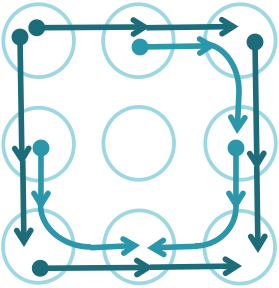
\includegraphics[width=0.31\textwidth]{pics/analysis/3gram1.png}
	    }
	    \subfigure{
	      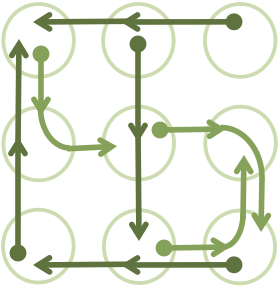
\includegraphics[width=0.31\textwidth]{pics/analysis/3gram2.png}
	    }
	    \subfigure{
	      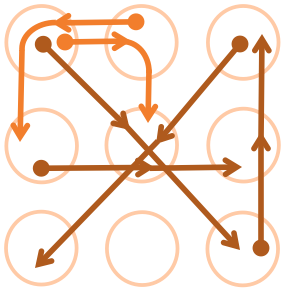
\includegraphics[width=0.31\textwidth]{pics/analysis/3gram3.png}
	    }
	    \caption{Most common 3-gram to less common 3-gram}
	    \label{fig:3gram}
	  \end{figure}

	\clearpage
	\subsection{The Impact of Using Latin Square} \label{sec:latinsquareimpact}

		%Figure: Percentage of times the pattern orders occurred
		\begin{figure}[H]
      \centering
      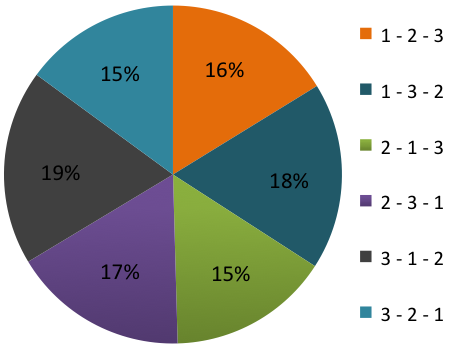
\includegraphics[scale=0.5]{pics/analysis/patternOrder.png}
      \caption{Percentage of times the pattern orders occurred}
      \label{fig:patternOrder}
    \end{figure}

